%%%%%%%%%%%%%%%%%%%%%%%%%%%%%%%%%%%%%%%%%%%%%%%%%%%%%%%%%%%%%%%%%%
%%  ~ Trabajo de Fin de Grado - Universidad de Vigo (ESEI) ~    %%
%% Autor: Diego Enrique Fontán Lorenzo                          %%
%% Tutor: Miguel Ramón Díaz-Cacho Medina                        %%
%% Convocatoria: Julio 2020/21                                  %%
%% Título: Framework de automatización de auditorías Red Team   %%
%%%%%%%%%%%%%%%%%%%%%%%%%%%%%%%%%%%%%%%%%%%%%%%%%%%%%%%%%%%%%%%%%%

%%%%%%%%%%%%%%%%%%%%%%%%%%%%%
%% Planification
%%%%%%%%%%%%%%%%%%%%%%%%%%%%%

\chapter{Planificación y seguimiento} \label{cap:planification}

En este capítulo se detalla el la metodología de trabajo seguida para la correcta realización del mismo, así como la planificación inicial, la descripción de las fases, la recogida de requisitos y las desviaciones respecto al plan sufridas durante el proceso de desarrollo.\n

%%%%%%%%%%%%%%%%%%%%%%%%%%%%%
%% Methodology
%%%%%%%%%%%%%%%%%%%%%%%%%%%%%

\section{Metodología de trabajo} \label{sec:methodology}

A continuación se explican las metodologías utilizadas a lo largo de la vida del desarrollo de este proyecto.\sn

Dichas metodologías han sido escogidas acorde a una serie de características derivadas de la naturaleza de la aplicación desarrollada, así como las habilidades y recursos disponibles por parte del autor de este documento.\n

\subsection{Metodología \textit{eXtreme Programming}} \label{sub:methoXP}

Para el desarrollo del proyecto se ha optado por implementar la metodología de Programación Extrema (o \textit{eXtreme Programming}).\sn

Catalogada como una metodología ágil, tiene como base la simplicidad y adaptabilidad, en vez de la previsibilidad. Esto permite que sea más natural hacer cambios sobre la marcha en los requisitos, en vez de tratar de definirlos todos al comienzo del proyecto. Es decir, conforme avance el proyecto, se adaptará el código a las necesidades que vayan surgiendo.\sn

\subsubsection{Características} \label{subsub:methoXPcaract}

Sus principales características son las siguientes:\sn

- Se diseña y construye una base sólida sobre la que añadir nuevas características, mediante un \textbf{desarrollo iterativo e incremental}.\sn

- Las capturas de requisitos deben ser escritas de manera breve y usando lenguaje natural por el cliente. A cada una de estas capturas se le conoce con el nombre de \textbf{historias de usuario}. Normalmente generan una nueva funcionalidad del sistema y deben ser independientes entre sí.\n

- Apuesta por mantener el \textbf{código lo más simplificado posible}, realizando una refractorización del mismo siempre que el desarrollador lo considere adecuado.\sn

- Antes de desarrollar cualquier funcionalidad nueva, se debe establecer un conjunto de objetivos, así como una \textbf{batería de pruebas unitarias}, preferiblemente automatizadas.\sn

- Antes de generar una nueva característica, es necesario \textbf{corregir todos los errores detectados en la iteración actual}, además de revisar y documentar cada una de las pruebas unitarias.\sn

- Se prioriza generar la \textbf{documentación de manera} integrada en los archivos fuente del \textit{software} y de forma simultánea al desarrollo, de manera que no existan iteraciones con segmentos de código sin documentar.\sn

- La \textbf{integración del cliente como parte del equipo} es necesaria para saber si el requerimiento cumple con las expectativas.\sn

- Se recomienda la \textbf{programación en parejas}, donde ambos integrantes comparten las actividades y responsabilidades referentes a un mismo código o proyecto.\n

\subsubsection{Limitaciones} \label{subsub:methoXPlimit}

Si bien la metodología expuesta encaja con el proyecto propuesto, no todas las características descritas en el apartado \ref{subsub:methoXPcaract} se ajustan a las restricciones inherentes a un Trabajo de Fin de Grado.\sn

En este caso concreto, el desarrollo de la aplicación no sigue la recomendación de la programación en parejas. Todo el proceso ha sido llevado a cabo por una única persona (el autor de este documento).\sn

Por otro lado, debido a que el cliente interesado en el producto no puede definirse con exactitud\footnote{Dependiendo de la opinión personal de cada lector, el cliente podría considerarse la propia Universidad, el tutor del proyecto o el público objetivo del trabajo, entre otros.}, se ha designado que sea el tutor del proyecto quien se encargue este rol, teniendo en cuenta las limitaciones de horarios y medios del mismo. El resto de roles pertenecientes a un equipo basado en esta metodología (\textit{Tester}, \textit{Coach}, \textit{Manager}...) recaen bajo el autor del trabajo.\sn

Por último, también será el autor quien genere gran parte de las historias de usuario, dado que se trata de un proyecto propio, el cual no ha sido propuesto por el tutor ni la Universidad.

\subsection{Anexo: Metodología \textit{SCRUM}} \label{sub:methoSCRUM}

Debido a que la documentación generada usando la metodología propuesta en el apartado \ref{sub:methoXP} no contempla de manera detallada la planificación del trabajo mediante la distribución en fases y tareas propias de un Trabajo de Fin de Grado, se ha optado por complementar este paradigma con otro proceso alternativo: la metodología \textit{SCRUM}.\sn

\subsubsection{Características} \label{subsub:methoSCRUMcaract}

Las características implementadas en este proyecto son:\sn

- El desarrollo incremental de los requisitos del proyecto se organiza en \textbf{bloques temporales cortos y fijos}.\sn

- Se establecen \textbf{tiempos máximos para lograr objetivos}.\sn

- \textbf{Se agrupan las tareas independientes en \textit{sprints}}, que a su vez harán de iteraciones.\sn

Dichas características son aplicadas solamente para la documentación del proyecto, dado que el desarrollo se llevará a cabo respecto a lo mencionado en el apartado \ref{sub:methoXP}.\n

%%%%%%%%%%%%%%%%%%%%%%%%%%%%%
%% Initial plan
%%%%%%%%%%%%%%%%%%%%%%%%%%%%%

\section{Planificación inicial} \label{sec:initialplan}

El desarrollo de la aplicación se ha dividido en ocho partes, con una estimación temporal asociada a cada una de ellas en función de la carga de trabajo \tab{initialplan}, con jornadas de ocho horas y semanas laborables de cinco días.\sn

\begin{table}[ht]
    \begin{center}
        \begin{tabular}{| l | c |}
            \hline
            \textbf{Iteración} & \textbf{Estimación} (en horas) \\
            \hline
            Investigación inicial                   & 32.0   \\ \hline
            Especificación de requisitos            & 16.0   \\ \hline
            Diseño del \textit{software}            & 24.0   \\ \hline
            \textit{Sprint} 1: Implementación de la interfaz & 80.0  \\ \hline
            \textit{Sprint} 2: Implementación de la \textit{API}      & 48.0   \\ \hline
            \textit{Sprint} 3: Implementación de los nodos   & 40.0   \\ \hline
            \textit{Sprint} 4: Integración del sistema       & 24.0   \\ \hline
            Elaboración del documento               & 96.0  \\ \hline
            \textbf{Total}                          & 360.0 \\ \hline
        \end{tabular}
    \end{center}
    \caption{Estimación temporal según la planificación inicial.}
    \label{tab:initialplan}
\end{table}
\vspace{1cm}

\subsection{Diagrama de Gantt} \label{sub:gantt}

A continuación se muestra la planificación temporal mediante un cronograma \fig{gantt}. El eje horizontal está asociado con el marco del tiempo (en días) y, el vertical, con cada una de las iteraciones.\sn

\begin{figure}[h]
    \centering
    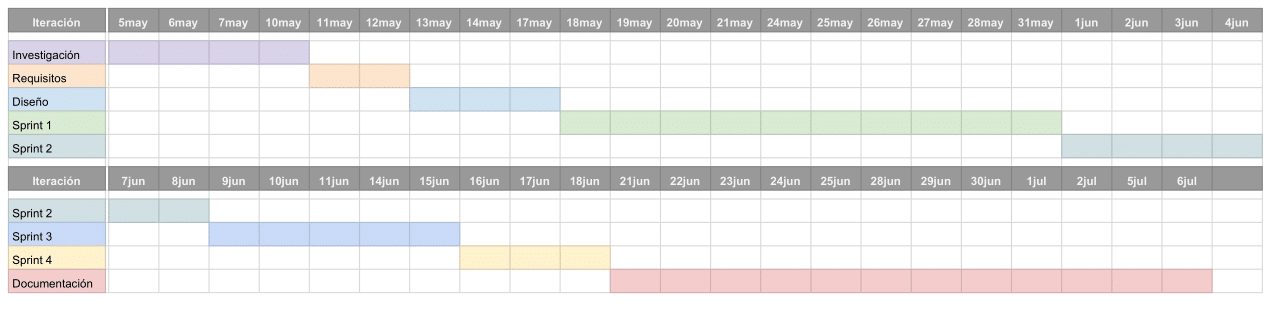
\includegraphics[width=15cm]{img/tables/08_Planned-Gantt.png}
    \caption{Diagrama de Gantt.}
    \label{fig:gantt}
\end{figure}

%%%%%%%%%%%%%%%%%%%%%%%%%%%%%
%% Phases
%%%%%%%%%%%%%%%%%%%%%%%%%%%%%

\section{Descripción de las fases} \label{sec:phases}

En este punto se procede a detallar cada una de las iteraciones descritas en el apartado \ref{sec:initialplan}. Además, por cada iteración, se definirán una serie de subtareas junto a su estimación temporal.\n

\subsection{Investigación inicial} \label{sub:initialinv}

Primera fase del proceso de desarrollo mediante la cual se realizará el estudio del arte, tomando como antecedentes aquellos proyectos que compartan características similares a la idea propuesta, ya sea en su motivación o en su implementación. Durante esta fase también se valorarán todos los conceptos relativos a lenguajes de programación, protocolos, patrones de diseño y metodologías que puedan ser objeto de interés durante el desarrollo.\sn

Las tareas asociadas a esta fase son:\sn

\begin{table}[ht]
    \begin{center}
        \begin{tabular}{| l | c |}
            \hline
            \textbf{Tarea} & \textbf{Estimación} (en horas) \\
            \hline
            Investigación sobre \textit{software} similar & 8.0 \\ \hline
            Investigación técnica   & 12.0 \\ \hline
            Investigación legal     & 4.0 \\ \hline
            Documentación relativa a ciberseguridad & 8.0 \\ \hline
            \textbf{Total}          & 32.0 \\ \hline
        \end{tabular}
    \end{center}
    \caption{Tareas y estimación temporal de la investigación inicial.}
    \label{tab:phase1}
\end{table}

\subsection{Especificación de requisitos} \label{sub:requirements}

La fase de especificación de requisitos consiste en la creación de las historias de usuario iniciales, las cuales formarán el núcleo de la aplicación. También se encargará de definir las herramientas necesarias para la realización del trabajo.\sn

Las tareas asociadas a esta fase son:\sn

\begin{table}[ht]
    \begin{center}
        \begin{tabular}{| l | c |}
            \hline
            \textbf{Tarea} & \textbf{Estimación} (en horas) \\
            \hline
            Definición de las historias de usuario  & 8.0 \\ \hline
            Definición de tecnologías y lenguajes   & 4.0 \\ \hline
            Planificación de los \textit{sprints}   & 4.0 \\ \hline
            \textbf{Total}                          & 16.0 \\ \hline
        \end{tabular}
    \end{center}
    \caption{Tareas y estimación temporal de la especificación de requisitos.}
    \label{tab:phase2}
\end{table}

\subsection{Diseño de la aplicación} \label{sub:appdesign}

En esta fase se valorará la arquitectura inicial de la aplicación. Es necesaria para concretar las bases sobre las que se comenzará a desarrollar el programa. Aún así, al tratarse de la metodología \textit{eXtreme Programming}, es posible que ésta se transforme a lo largo de todo el proceso de desarrollo.\sn

Las tareas asociadas a esta fase son:\sn

\begin{table}[ht]
    \begin{center}
        \begin{tabular}{| l | c |}
            \hline
            \textbf{Tarea} & \textbf{Estimación} (en horas) \\
            \hline
            Diseño de la arquitectura               & 12.0 \\ \hline
            Bocetaje de posibles flujos de datos    & 8.0 \\ \hline
            Bocetaje de la interfaz                 & 4.0 \\ \hline
            \textbf{Total}                          & 24.0 \\ \hline
        \end{tabular}
    \end{center}
    \caption{Tareas y estimación temporal del diseño de la aplicación.}
    \label{tab:phase3}
\end{table}

\subsection{\textit{Sprint} 1 - Implementación de la interfaz} \label{sub:sprint1}

El primer \textit{sprint} está dedicado a la creación de la interfaz visual. Se encargará de implementar cómo interpretará la aplicación el flujo de datos y todo lo referente a la interacción con el usuario.\sn

A pesar de tratarse de una aplicación híbrida, y al contrario que en los procesos de desarrollo de aplicaciones para escritorio (donde la interfaz generalmente es lo último en implementarse), se ha optado por una aproximación similar al proceso de desarrollo web, en el que el \textit{frontend} es el protagonista.\n

Las tareas asociadas a esta fase son:\sn

\begin{table}[ht]
    \begin{center}
        \begin{tabular}{| l | c |}
            \hline
            \textbf{Tarea} & \textbf{Estimación} (en horas) \\
            \hline
            Creación de pruebas unitarias       & 8.0 \\ \hline
            Diseño del modelo de flujo de datos & 36.0 \\ \hline
            Implementación del flujo de datos   & 16.0 \\ \hline
            Diseño de la interfaz gráfica       & 20.0 \\ \hline
            \textbf{Total}                      & 80.0 \\ \hline
        \end{tabular}
    \end{center}
    \caption{Tareas y estimación temporal de la implementación de la interfaz.}
    \label{tab:phase4}
\end{table}

\subsection{\textit{Sprint} 2 - Implementación de la \textit{API}} \label{sub:sprint2}

El segundo \textit{sprint} está dedicado a la creación de la \textit{API}. Se encargará de crear el servidor \textit{HTTP}, definir el enrutamiento e implementar las peticiones a terceros.\sn

Las tareas asociadas a esta fase son:\sn

\begin{table}[ht]
    \begin{center}
        \begin{tabular}{| l | c |}
            \hline
            \textbf{Tarea} & \textbf{Estimación} (en horas) \\
            \hline
            Creación de pruebas unitarias       & 8.0 \\ \hline
            Implementación del servidor         & 12.0 \\ \hline
            Implementación del \textit{router}  & 12.0 \\ \hline
            Implementación de los \textit{middlewares} & 4.0 \\ \hline
            Implementación de las acciones relativas a terceros & 12.0 \\ \hline
            \textbf{Total}                          & 48.0 \\ \hline
        \end{tabular}
    \end{center}
    \caption{Tareas y estimación temporal de la implementación de la \textit{API}.}
    \label{tab:phase5}
\end{table}

\subsection{\textit{Sprint} 3 - Implementación de los nodos} \label{sub:sprint3}

El tercer \textit{sprint} consta de la definición de un estándar asociado a la creación de los nodos, así como la propia creación de varios nodos de ejemplo.\sn

Los tipos de nodos resultantes fruto de esta iteración formarán parte del cuerpo de la aplicación, pero se dedicará más tiempo y recursos a una sólida estandarización, con el objetivo de proporcionar a la comunidad la habilidad de diseñar, crear y compartir sus propios nodos.\sn

Las tareas asociadas a esta fase son:\sn

\begin{table}[ht]
    \begin{center}
        \begin{tabular}{| l | c |}
            \hline
            \textbf{Tarea} & \textbf{Estimación} (en horas) \\
            \hline
            Creación de pruebas unitarias       & 8.0 \\ \hline
            Estandarización de los nodos        & 16.0 \\ \hline
            Implementación de los nodos         & 8.0 \\ \hline
            Creación de varios nodos de ejemplo & 8.0 \\ \hline
            \textbf{Total}                      & 40.0 \\ \hline
        \end{tabular}
    \end{center}
    \caption{Tareas y estimación temporal de la implementación de los nodos.}
    \label{tab:phase6}
\end{table}

\subsection{\textit{Sprint} 4 - Integración del sistema} \label{sub:sprint4}

El último \textit{sprint} corresponde a la interconexión de los módulos desarrollados en las etapas anteriores del desarrollo. Será el encargado de unificar la interfaz gráfica con el servidor, además de preparar los archivos necesarios para su correcta distribución.\sn

Las tareas asociadas a esta fase son:\sn

\begin{table}[ht]
    \begin{center}
        \begin{tabular}{| l | c |}
            \hline
            \textbf{Tarea} & \textbf{Estimación} (en horas) \\
            \hline
            Creación de pruebas unitarias       & 8.0 \\ \hline
            Interconexión de los módulos        & 12.0 \\ \hline
            Creación de los archivos y \textit{scripts} de distribución         & 4.0 \\ \hline
            \textbf{Total}                      & 24.0 \\ \hline
        \end{tabular}
    \end{center}
    \caption{Tareas y estimación temporal de la integración del sistema.}
    \label{tab:phase7}
\end{table}

\subsection{Elaboración de la documentación} \label{sub:makedoc}

Tras el desarrollo del proyecto, el último marco temporal está reservado para la maquetación del documento actual, así como de los Anexos y demás archivos referentes a la documentación del Trabajo de Fin de Grado.\sn

Las tareas asociadas a esta fase son:\sn

\begin{table}[ht]
    \begin{center}
        \begin{tabular}{| l | c |}
            \hline
            \textbf{Tarea} & \textbf{Estimación} (en horas) \\
            \hline
            Memoria del proyecto    & 80.0 \\ \hline
            Anexos                  & 16.0 \\ \hline
            \textbf{Total}          & 96.0 \\ \hline
        \end{tabular}
    \end{center}
    \caption{Tareas y estimación temporal de la elaboración del documento.}
    \label{tab:phase8}
\end{table}

%%%%%%%%%%%%%%%%%%%%%%%%%%%%%
%% Requirements
%%%%%%%%%%%%%%%%%%%%%%%%%%%%%

\section{Historias de usuario} \label{sec:userrequirements}

Durante la tarea descrita en el apartado \ref{sub:requirements} y en relación a la metodología usada en este proyecto (ver apartado \ref{sec:methodology}), los requisitos de la aplicación se han definido usando \textbf{historias de usuario}, que actuarán a su vez de \textit{Product  Backlog}\footnote{Listado  de todas  las  tareas  que  se  pretenden  hacer  durante  el desarrollo del proyecto.} (relativo a la metodología \textit{SCRUM}). A continuación, se detallan cada una de ellas de manera numerada siguiendo el formato \textbf{HUXX}, donde \textit{XX} corresponde a un número de identificación arbitrario\footnote{El orden de las historias de usuario no viene determinado por su orden de implementación. Para reflejar este aspecto, se ha optado por asociar cada una de ellas a los \textit{sprints} definidos en el apartado \ref{tab:initialplan}.}.\sn

Todas las historias de usuario deben comenzar por el texto ``Deseo \ldots'' y tienen una prioridad asociada del 1 al 100 (siendo 1 la más baja y 100 la más alta).\sn

Los requisitos iniciales especificados son:\sn

\begin{table}[H]
    \begin{center}
        \begin{tabularx}{\textwidth}{| l | X |}
            \hline
            \textbf{ID}             & HU01 \\ \hline
            \textbf{Título}         & Deseo que la aplicación tenga interfaz gráfica \\ \hline
            \textbf{Descripción}    & La aplicación debe poder ser manejable mediante el uso del ratón \\ \hline
            \textbf{Prioridad}      & 90 \\ \hline
            \textbf{Iteración}      & \textit{Sprint} 1 \\ \hline
        \end{tabularx}
    \end{center}
    \caption{Historia de usuario -- 01.}
    \label{tab:hu01}
\end{table}

\begin{table}[H]
    \begin{center}
        \begin{tabularx}{\textwidth}{| l | X |}
            \hline
            \textbf{ID}             & HU02 \\ \hline
            \textbf{Título}         & Deseo que sea capaz de ejecutar tareas propias de un \textit{pentesting} \\ \hline
            \textbf{Descripción}    & La aplicación debe poder realizar controles asociados a una auditoría \\ \hline
            \textbf{Prioridad}      & 99 \\ \hline
            \textbf{Iteración}      & \textit{Sprint} 2\\ \hline
        \end{tabularx}
    \end{center}
    \caption{Historia de usuario -- 02.}
    \label{tab:hu02}
\end{table}

\begin{table}[H]
    \begin{center}
        \begin{tabularx}{\textwidth}{| l | X |}
            \hline
            \textbf{ID}             & HU03 \\ \hline
            \textbf{Título}         & Deseo que se puedan declarar varios activos a auditar \\ \hline
            \textbf{Descripción}    & La aplicación debe asociar tareas a uno o más objetivos concretos \\ \hline
            \textbf{Prioridad}      & 25 \\ \hline
            \textbf{Iteración}      & \textit{Sprint} 2\\ \hline
        \end{tabularx}
    \end{center}
    \caption{Historia de usuario -- 03.}
    \label{tab:hu03}
\end{table}

\begin{table}[H]
    \begin{center}
        \begin{tabularx}{\textwidth}{| l | X |}
            \hline
            \textbf{ID}             & HU04 \\ \hline
            \textbf{Título}         & Deseo tener una lista de controles de seguridad por defecto \\ \hline
            \textbf{Descripción}    & La aplicación debe proporcionar un catálogo de tareas habituales \\ \hline
            \textbf{Prioridad}      & 60 \\ \hline
            \textbf{Iteración}      & \textit{Sprint} 3\\ \hline
        \end{tabularx}
    \end{center}
    \caption{Historia de usuario -- 04.}
    \label{tab:hu04}
\end{table}

\begin{table}[H]
    \begin{center}
        \begin{tabularx}{\textwidth}{| l | X |}
            \hline
            \textbf{ID}             & HU05 \\ \hline
            \textbf{Título}         & Deseo poder crear mis propios controles de seguridad \\ \hline
            \textbf{Descripción}    & La aplicación debe poder interpretar tareas definidas bajo un estándar \\ \hline
            \textbf{Prioridad}      & 40 \\ \hline
            \textbf{Iteración}      & \textit{Sprint} 3 \\ \hline
        \end{tabularx}
    \end{center}
    \caption{Historia de usuario -- 05.}
    \label{tab:hu05}
\end{table}

\begin{table}[H]
    \begin{center}
        \begin{tabularx}{\textwidth}{| l | X |}
            \hline
            \textbf{ID}             & HU06 \\ \hline
            \textbf{Título}         & Deseo poder ejecutar controles de manera condicional \\ \hline
            \textbf{Descripción}    & Las tareas deben poder compartir datos entre sí \\ \hline
            \textbf{Prioridad}      & 70 \\ \hline
            \textbf{Iteración}      & \textit{Sprint} 1\\ \hline
        \end{tabularx}
    \end{center}
    \caption{Historia de usuario -- 06.}
    \label{tab:hu06}
\end{table}

\begin{table}[H]
    \begin{center}
        \begin{tabularx}{\textwidth}{| l | X |}
            \hline
            \textbf{ID}             & HU07 \\ \hline
            \textbf{Título}         & Deseo poder definir el momento en el que se ejecutan las tareas \\ \hline
            \textbf{Descripción}    & La aplicación debe soportar señales de evento \\ \hline
            \textbf{Prioridad}      & 65 \\ \hline
            \textbf{Iteración}      & \textit{Sprint} 1\\ \hline
        \end{tabularx}
    \end{center}
    \caption{Historia de usuario -- 07.}
    \label{tab:hu07}
\end{table}


\begin{table}[H]
    \begin{center}
        \begin{tabularx}{\textwidth}{| l | X |}
            \hline
            \textbf{ID}             & HU08 \\ \hline
            \textbf{Título}         & Deseo poder configurar controles en base a parámetros \\ \hline
            \textbf{Descripción}    & Las tareas similares deben fusionarse en una única tarea personalizable \\ \hline
            \textbf{Prioridad}      & 10 \\ \hline
            \textbf{Iteración}      & \textit{Sprint} 3\\ \hline
        \end{tabularx}
    \end{center}
    \caption{Historia de usuario -- 08.}
    \label{tab:hu08}
\end{table}


\begin{table}[H]
    \begin{center}
        \begin{tabularx}{\textwidth}{| l | X |}
            \hline
            \textbf{ID}             & HU09 \\ \hline
            \textbf{Título}         & Deseo poder guardar plantillas de auditorías \\ \hline
            \textbf{Descripción}    & La aplicación debe proporcionar un sistema de guardado \\ \hline
            \textbf{Prioridad}      & 8 \\ \hline
            \textbf{Iteración}      & \textit{Sprint} 1\\ \hline
        \end{tabularx}
    \end{center}
    \caption{Historia de usuario -- 09.}
    \label{tab:hu09}
\end{table}

\begin{table}[H]
    \begin{center}
        \begin{tabularx}{\textwidth}{| l | X |}
            \hline
            \textbf{ID}             & HU10 \\ \hline
            \textbf{Título}         & Deseo poder compartir plantillas de auditorías \\ \hline
            \textbf{Descripción}    & La carga de plantillas debe estar sujeta a un control de versiones \\ \hline
            \textbf{Prioridad}      & 5 \\ \hline
            \textbf{Iteración}      & \textit{Sprint} 1\\ \hline
        \end{tabularx}
    \end{center}
    \caption{Historia de usuario -- 10.}
    \label{tab:hu10}
\end{table}

\begin{table}[H]
    \begin{center}
        \begin{tabularx}{\textwidth}{| l | X |}
            \hline
            \textbf{ID}             & HU11 \\ \hline
            \textbf{Título}         & Deseo que el programa no tenga dependencias \\ \hline
            \textbf{Descripción}    & La ejecución no debe depender de archivos o programas de terceros \\ \hline
            \textbf{Prioridad}      & 85 \\ \hline
            \textbf{Iteración}      & \textit{Sprint} 4\\ \hline
        \end{tabularx}
    \end{center}
    \caption{Historia de usuario -- 11.}
    \label{tab:hu11}
\end{table}

\begin{table}[H]
    \begin{center}
        \begin{tabularx}{\textwidth}{| l | X |}
            \hline
            \textbf{ID}             & HU12 \\ \hline
            \textbf{Título}         & Deseo que el programa sea multiplataforma \\ \hline
            \textbf{Descripción}    & El binario debe soportar sistemas operativos y arquitecturas populares\\ \hline
            \textbf{Prioridad}      & 80 \\ \hline
            \textbf{Iteración}      & \textit{Sprint} 4\\ \hline
        \end{tabularx}
    \end{center}
    \caption{Historia de usuario -- 12.}
    \label{tab:hu12}
\end{table}

\begin{table}[H]
    \begin{center}
        \begin{tabularx}{\textwidth}{| l | X |}
            \hline
            \textbf{ID}             & HU13 \\ \hline
            \textbf{Título}         & Deseo poder auditar objetivos que no pertenezcan a mi red local \\ \hline
            \textbf{Descripción}    & La aplicación debe poder realizar peticiones a través de Internet \\ \hline
            \textbf{Prioridad}      & 95 \\ \hline
            \textbf{Iteración}      & \textit{Sprint} 2\\ \hline
        \end{tabularx}
    \end{center}
    \caption{Historia de usuario -- 13.}
    \label{tab:hu13}
\end{table}

\begin{table}[H]
    \begin{center}
        \begin{tabularx}{\textwidth}{| l | X |}
            \hline
            \textbf{ID}             & HU14 \\ \hline
            \textbf{Título}         & Deseo poder recopilar información de fuentes abiertas \\ \hline
            \textbf{Descripción}    & La aplicación debe poder obtener datos de servicios concretos \\ \hline
            \textbf{Prioridad}      & 20 \\ \hline
            \textbf{Iteración}      & \textit{Sprint} 2\\ \hline
        \end{tabularx}
    \end{center}
    \caption{Historia de usuario -- 14.}
    \label{tab:hu14}
\end{table}

\begin{table}[H]
    \begin{center}
        \begin{tabularx}{\textwidth}{| l | X |}
            \hline
            \textbf{ID}             & HU15 \\ \hline
            \textbf{Título}         & Deseo que los controles estén agrupados por categorías \\ \hline
            \textbf{Descripción}    & Las tareas deben pertenecer a una categoría concreta \\ \hline
            \textbf{Prioridad}      & 2 \\ \hline
            \textbf{Iteración}      & \textit{Sprint} 3\\ \hline
        \end{tabularx}
    \end{center}
    \caption{Historia de usuario -- 15.}
    \label{tab:hu15}
\end{table}

\begin{table}[H]
    \begin{center}
        \begin{tabularx}{\textwidth}{| l | X |}
            \hline
            \textbf{ID}             & HU16 \\ \hline
            \textbf{Título}         & Deseo poder encontrar rápidamente un control concreto \\ \hline
            \textbf{Descripción}    & Las tareas se podrán filtrar por nombre o palabras clave \\ \hline
            \textbf{Prioridad}      & 7 \\ \hline
            \textbf{Iteración}      & \textit{Sprint} 3\\ \hline
        \end{tabularx}
    \end{center}
    \caption{Historia de usuario -- 16.}
    \label{tab:hu16}
\end{table}

\begin{table}[H]
    \begin{center}
        \begin{tabularx}{\textwidth}{| l | X |}
            \hline
            \textbf{ID}             & HU17 \\ \hline
            \textbf{Título}         & Deseo poder visualizar los resultados de múltiples maneras \\ \hline
            \textbf{Descripción}    & La aplicación proporcionará diferentes tipos de nodos de salida \\ \hline
            \textbf{Prioridad}      & 6 \\ \hline
            \textbf{Iteración}      & \textit{Sprint} 3\\ \hline
        \end{tabularx}
    \end{center}
    \caption{Historia de usuario -- 17.}
    \label{tab:hu17}
\end{table}

\begin{table}[H]
    \begin{center}
        \begin{tabularx}{\textwidth}{| l | X |}
            \hline
            \textbf{ID}             & HU18 \\ \hline
            \textbf{Título}         & Deseo que la aplicación cuente con mecanismos de protección \\ \hline
            \textbf{Descripción}    & La implementación deberá seguir ciertos estándares de seguridad \\ \hline
            \textbf{Prioridad}      & 75 \\ \hline
            \textbf{Iteración}      & \textit{Sprint} 4\\ \hline
        \end{tabularx}
    \end{center}
    \caption{Historia de usuario -- 18.}
    \label{tab:hu18}
\end{table}

%% Resumen de las historias de usuario segun su prioridad
% 099 - Deseo que sea capaz de ejecutar tareas propias de un pentesting
% 095 - Deseo poder auditar objetivos que no pertenezcan a mi red local
% 090 - Deseo que la aplicación tenga interfaz gráfica
% 085 - Deseo que el programa no tenga dependencias
% 080 - Deseo que el programa sea multiplataforma
% 075 - Deseo que la aplicación cuente con mecanismos de protección
% 070 - Deseo poder ejecutar controles de manera condicional
% 065 - Deseo poder definir el momento en el que se ejecutan las tareas
% 060 - Deseo tener una lista de controles de seguridad por defecto
% 040 - Deseo poder crear mis propios controles de seguridad
% 025 - Deseo que se puedan declarar uno más activos a auditar
% 020 - Deseo poder recopilar información de fuentes abiertas
% 010 - Deseo poder configurar controles en base a parámetros
% 008 - Deseo poder guardar plantillas de auditorías
% 007 - Deseo poder encontrar rápidamente un control concreto
% 006 - Deseo poder visualizar los resultados de múltiples maneras
% 005 - Deseo poder compartir plantillas de auditorías
% 002 - Deseo que los controles estén agrupados por categorías

%%%%%%%%%%%%%%%%%%%%%%%%%%%%%
%% Tracking
%%%%%%%%%%%%%%%%%%%%%%%%%%%%%

\section{Seguimiento de la planificación} \label{sec:tracking}

El seguimiento se ha ejecutado utilizando la metodología \textit{Kanban} \cite{wikiKanban}, la cual también se denomina \textit{sistema de tarjetas}, pues en su implementación más sencilla se usan tarjetas sobre un tablero segmentado en tres partes fundamentales:\sn

- Tareas pendientes

- Tareas en curso

- Tareas finalizadas\sn

Según la metodología descrita en el apartado \ref{sub:methoXP}, el segmento de \textit{Tareas en curso} solamente deberá contener un máximo de una tarea. Además, se han agrupado las historias de usuario según el \textit{sprint} al que pertenecen, mediante un código de colores, siguiendo la especificación del apartado \ref{sec:userrequirements} \fig{trellokanban}.\sn

\begin{figure}[h]
    \centering
    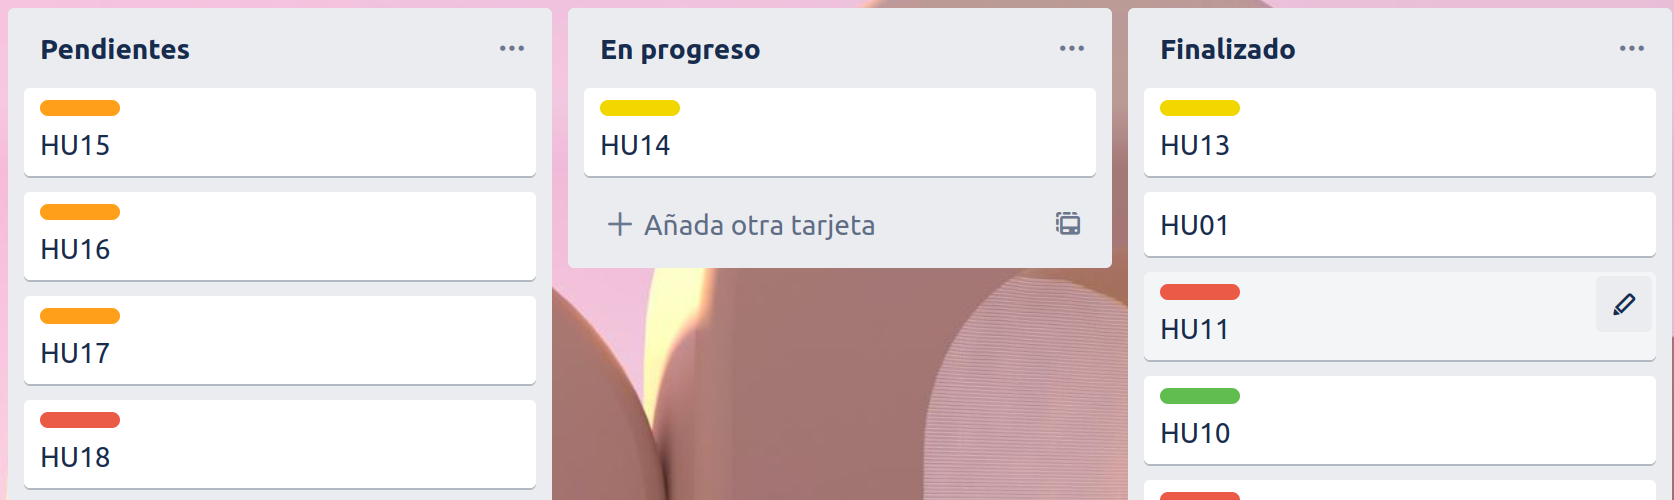
\includegraphics[width=14cm]{img/tables/09_Trello.png}
    \caption{Estado del tablero \textit{Kanban} durante el desarrollo.}
    \label{fig:trellokanban}
\end{figure}

%%%%%%%%%%%%%%%%%%%%%%%%%%%%%
%% Variations
%%%%%%%%%%%%%%%%%%%%%%%%%%%%%

\section{Desviaciones respecto a la planificación inicial} \label{sec:variations}

A lo hora de desarrollar el proyecto, se han observado algunas irregularidades en relación a los tiempos marcados en el apartado \ref{sec:initialplan}. Dichas irregularidades son comunes al realizar aplicaciones debido a que la guía temporal que ofrece la planificación inicial, aunque contemple la corrección de errores y contratiempos, se trata solamente de una valoración subjetiva de la dimensión de las tareas.\sn

A continuación se detallan las desviaciones respecto a la planificación que se han ido encontrado a lo largo del desarrollo.\sn

\subsection{Investigación inicial} \label{sub:varinvestigation}

Esta fase se consiguió completar un 400\% más rápido de lo previsto, debido a que el autor contaba con experiencia previa relativa a temas de ciberseguridad, así como sus conceptos legales, además del conocimiento sobre la existencia de herramientas similares.\n

\subsection{\textit{Sprint} 1 - Implementación de la interfaz} \label{sub:varsprint1}

Durante la implementación de la interfaz, se encontraron varios errores asociados al paradigma de programación basado en flujos de datos, que retrasaron el \textit{sprint} seis días laborables más de lo previsto (48 horas). Esto fue debido a una incompatibilidad entre el diseño y el desarrollo que obligó a tener que pausar la tarea en curso y rediseñar por completo el modelo de flujo de datos.\sn

Para compensar este imprevisto, se optó por prescindir de la creación de pruebas unitarias al comienzo de cada \textit{sprint}, reemplazándolas por pruebas manuales en paralelo con el desarrollo.\n

\subsection{Elaboración de la documentación} \label{sub:vardoc}

Por último, se decidió dedicar 4 horas más a la elaboración de este documento, durante las cuales se diseñó una plantilla haciendo uso de herramientas especializadas en la creación de documentos científicos (ver apartado \ref{sec:latex}), con el fin de mejorar la calidad de la documentación.\n

%%%%%%%%%%%%%%%%%%%%%%%%%%%%%
%% Result
%%%%%%%%%%%%%%%%%%%%%%%%%%%%%

\section{Resultado de la planificación} \label{sec:resultplan}

Tras la realización del proyecto, se ha analizado el resultado de la planificación inicial (Apartado \ref{sec:initialplan}).\sn

A pesar los imprevistos detallados en el apartado \ref{sec:variations}, la variación total del tiempo se redujo a cuatro horas de diferencia, excediendo la fecha de finalización un día más de lo previsto \tab{realplan}.\sn

\begin{table}[H]
    \begin{center}
        \begin{tabular}{| l | c | c |}
            \hline
            \textbf{Iteración} & \textbf{T. estimado} (en horas) &  \textbf{T. real} (en horas) \\
            \hline
            Investigación inicial           & 32.0 & \cellcolor{green!10} 8.0 \\ \hline
            Especificación de requisitos    & 16.0 & 16.0 \\ \hline
            Diseño del \textit{software}    & 24.0 & 24.0 \\ \hline
            \textit{Sprint} 1: Implementación de la interfaz & 80.0 & \cellcolor{red!10} 128.0 \\ \hline
            \textit{Sprint} 2: Implementación de la \textit{API} & 48.0 & \cellcolor{green!10} 40.0 \\ \hline
            \textit{Sprint} 3: Implementación de los nodos & 40.0 & \cellcolor{green!10} 32.0 \\ \hline
            \textit{Sprint} 4: Integración del sistema & 24.0 & \cellcolor{green!10} 16.0 \\ \hline
            Elaboración del documento       & 96.0 & \cellcolor{red!10} 100.0 \\ \hline
            \textbf{Total}                  & 360.0 & \cellcolor{red!10} 364.0  \\ \hline
        \end{tabular}
    \end{center}
    \caption{Estimación temporal real en comparación con la planificación inicial.}
    \label{tab:realplan}
\end{table}
\vspace{1cm}

\subsection{Diagrama de Gantt} \label{sub:realgantt}

A continuación se muestra el tiempo real dedicado mediante un cronograma \fig{realgantt}. El eje horizontal está asociado con el marco del tiempo y, el vertical, con cada una de las iteraciones. Además, también se resaltan las desviaciones respecto a la planificación inicial.\sn

\begin{figure}[H]
    \centering
    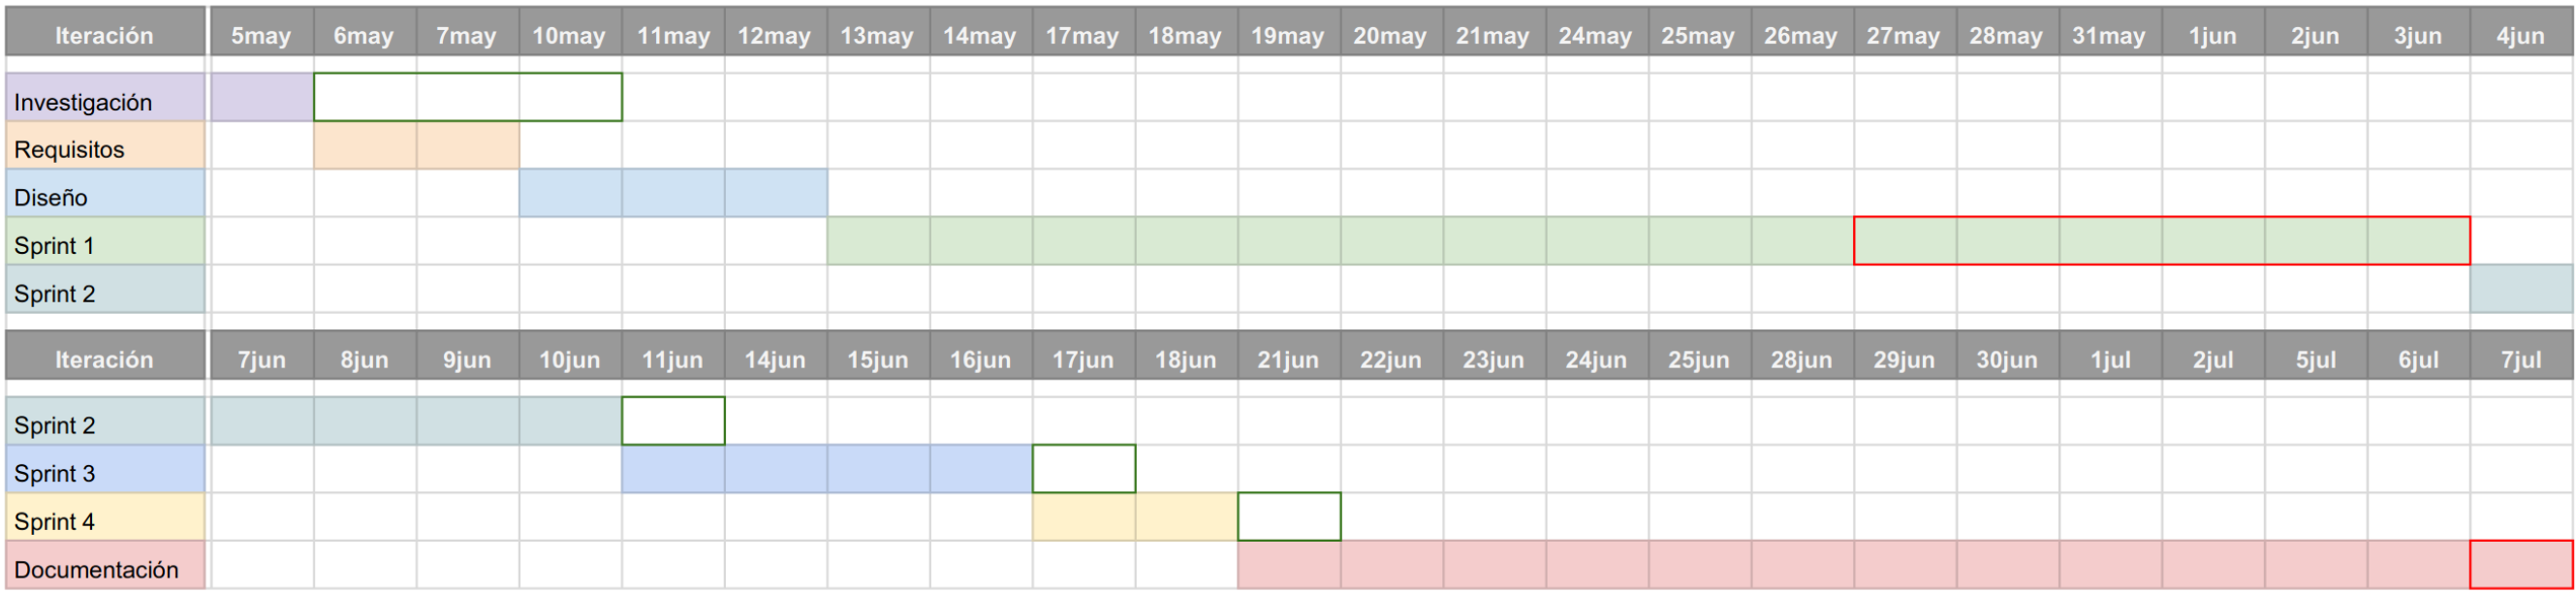
\includegraphics[width=15cm]{img/tables/10_Real-Gantt.png}
    \caption{Diagrama de Gantt resultante.}
    \label{fig:realgantt}
\end{figure}
